\begin{activity} \label{A:10.3.2a} 
We continue to consider the function $f$ defined by $f(x,y) = \sin(x) e^{-y}$.
    \ba
	\item  In Figure~\ref{F:10.3.fyy}, we see the trace of $f(x,y) = \sin(x) e^{-y}$ that has $x$ held constant with $x = 1.75$. 
\begin{figure}[ht]
  \begin{center}
    \includegraphics[scale=0.8]{figures/fig_10_3_fyy_1.eps}
    \includegraphics[scale=0.8]{figures/fig_10_3_fyy_2.eps}
    \includegraphics[scale=0.8]{figures/fig_10_3_fyy_3.eps}
  \end{center}
  \caption{The tangent lines to a trace with increasing $y$.}
  \label{F:10.3.fyy}
\end{figure}
Write a couple of sentences that describe whether the slope of the tangent lines to this curve increase or decrease as $y$ increases, and, after computing $f_{yy}(x,y)$, explain how this observation is related to the value of $f_{yy}(1.75,y)$.  Be sure to address the notion of concavity in your response.

	\item  In Figure~\ref{F:10.3.fxy}, we start to think about the mixed partial derivative, $f_{xy}$.  Here, we first hold $y$ constant to generate the first-order partial derivative $f_x$, and then we hold $x$ constant to compute $f_{xy}$.  This leads to first thinking about a trace with $x$ being constant, followed by slopes of tangent lines in the $y$-direction that slide along the original trace.  You might think of sliding your pencil down the trace with $x$ constant in a way that its slope indicates $(f_x)_y$ in order to further animate the three snapshots shown in the figure.
\begin{figure}[ht]
  \begin{center}
    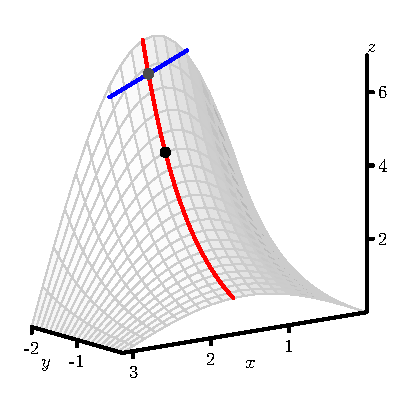
\includegraphics[scale=0.8]{figures/fig_10_3_fxy_1.eps}
    \includegraphics[scale=0.8]{figures/fig_10_3_fxy_2.eps}
    \includegraphics[scale=0.8]{figures/fig_10_3_fxy_3.eps}
  \end{center}
  \caption{The trace of $z = f(x,y) = \sin(x)e^{-y}$ with $x = 1.75$, along with tangent lines in the $y$-direction at three different points.}
  \label{F:10.3.fxy}
\end{figure}	
Based on Figure~\ref{F:10.3.fxy}, is $f_{xy}(1.75, -1.5)$ positive or negative?  Why?

	\item Determine the formula for $f_{xy}(x,y)$, and hence evaluate $f_{xy}(1.75, -1.5)$.  How does this value compare with your observations in (b)?
	
	\item We know that $f_{xx}(1.75, -1.5)$ measures the concavity of the $y = -1.5$ trace, and that $f_{yy}(1.75, -1.5)$ measures the concavity of the $x = 1.75$ trace.  What do you think $f_{xy}(1.75, -1.5)$ measures?
	
	\item On Figure~\ref{F:10.3.fxy}, sketch the trace with $y = -1.5$, and sketch three tangent lines whose slopes correspond to the value of $f_{yx}(x,-1.5)$ for three different values of $x$, the middle of which is $x = -1.5$.  Is $f_{yx}(1.75, -1.5)$ positive or negative?  Why?  What does $f_{yx}(1.75, -1.5)$ measure?


  \ea

\end{activity}
\begin{smallhint}

\end{smallhint}
\begin{bighint}

\end{bighint}
\begin{activitySolution}
\ba
\item The figures seem to indicate that the slopes of the tangent lines to the trace $f(1.75,y)$ increase as $y$ increases. Note that $\frac{d}{dy} f(1.75,y) = \frac{d}{dy} \sin(1.75) e^{-y} = -\sin(1.75) e^{-y}$, so as $y$ increases the slopes of the tangent lines become less negative. Note also that $\frac{d^2}{dy^2} f(1.75,y) = \sin(1.75)e^{-y}$ which is a decreasing function. This tells us that the $x=1.75$ trace is concave down. That means that the slopes of the tangent lines to the trace are increasing, but at a decreasing rate. This is reflected in the fact that the surface seems to be leveling off as $y$ increases. 

\item Based on the figure, the slopes of the tangent lines in the $x$ direction along the $x=1.75$ trace appear to be negative, but getting less negative as $y$ increases. So we expect $f_{xy}(1.75,-1.5)$ to be positive.  

\item Since $f_x(x,y) = \cos(x)e^{-y}$, we have $f_{xy} = -\cos(x)e^{-y}$. So $f_{xy}(1.75,-1.5) \approx 0.8$. This number is positive, as we discussed in the previous part. 

\item The quantity $f_{xy}(1.75,-1.5)$ tells us how much the slopes of the $x=1.75$ trace change as we increase $y$ from $-1.5$. Geometrically, we could describe $f_{xy}(1.75,-1.5)$ as telling us how much the surface ``twists" in the $y$ direction when $y=-1.5$ as we move along the $x=1.75$ trace. 

\item The sketches are shown below. Since $f_y(x,y) = -\sin(x)e^{-y}$, when $x$ exceeds $\frac{\pi}{2}$ and increases, $f_y(x,y)$ increases for fixed $y$. So we should expect $f_{yx}(1.75,-1.5)$ to be positive. In fact, $f_{yx}(1.75,-1.5) = 0.8$. The value of $f_{yx}(1.75,-1.5)$ measures how much the surface ``twists" in the $x$ direction when $x=1.75$ as we move along the $y=-1.5$ trace.  

   \begin{center}
      \resizebox{!}{2.0in}{\includegraphics{figures/fig_10_3_Act_2a_fyx_1.png}} \ \ \resizebox{!}{2.0in}{\includegraphics{figures/fig_10_3_Act_2a_fyx_2.png}} \ \ \resizebox{!}{2.0in}{\includegraphics{figures/fig_10_3_Act_2a_fyx_3.png}}
    \end{center}
\ea
\end{activitySolution}
\aftera
